\documentclass{article}
\usepackage{CJKutf8}
\usepackage{amsfonts}
\usepackage{fancyhdr}
\usepackage{comment}
\usepackage[a4paper, top=2.5cm, bottom=2.5cm, left=2.2cm, right=2.2cm]%
{geometry}
\usepackage{times}
\usepackage{amsmath}
\usepackage{changepage}
\usepackage{amssymb}
\usepackage{graphicx}
\usepackage{url}%
\setcounter{MaxMatrixCols}{30}
\newtheorem{theorem}{Theorem}
\newtheorem{acknowledgement}[theorem]{Acknowledgement}
\newtheorem{algorithm}[theorem]{Algorithm}
\newtheorem{axiom}{Axiom}
\newtheorem{case}[theorem]{Case}
\newtheorem{claim}[theorem]{Claim}
\newtheorem{conclusion}[theorem]{Conclusion}
\newtheorem{condition}[theorem]{Condition}
\newtheorem{conjecture}[theorem]{Conjecture}
\newtheorem{corollary}[theorem]{Corollary}
\newtheorem{criterion}[theorem]{Criterion}
\newtheorem{definition}[theorem]{Definition}
\newtheorem{example}[theorem]{Example}
\newtheorem{exercise}[theorem]{Exercise}
\newtheorem{lemma}[theorem]{Lemma}
\newtheorem{notation}[theorem]{Notation}
\newtheorem{problem}[theorem]{Problem}
\newtheorem{proposition}[theorem]{Proposition}
\newtheorem{remark}[theorem]{Remark}
\newtheorem{solution}[theorem]{Solution}
\newtheorem{summary}[theorem]{Summary}
\newenvironment{proof}[1][Proof]{\textbf{#1.} }{\ \rule{0.5em}{0.5em}}

\newcommand{\Q}{\mathbb{Q}}
\newcommand{\R}{\mathbb{R}}
\newcommand{\C}{\mathbb{C}}
\newcommand{\Z}{\mathbb{Z}}

\begin{document}

\title{BME2126 Spring 2024 Assignment 1}
\maketitle
\paragraph{Name:} 
\begin{CJK}{UTF8}{gbsn}
廖寒曦
\end{CJK}
\paragraph{Student ID:} 2023291025

\section*{Question}
Consider the function
$$f(x)=\frac{\sin(x)}{x^3}$$
Consider the first-order forward difference, second-order central difference, and fourth-order central-difference approximations to the first derivative. Plot the absolute value of the difference between the computed and exact derivative (i.e. the truncation error) at $x=4.0$ for different grid sizes ($\Delta x$) and show that the error changes with grid size as expected (order of accuracy). Employ at least five different grid sizes.

\subsection*{Answer}
The first-order forward difference approximation function of the original function is: $$\frac{\partial f(x)}{\partial x} = \frac{f(x+\Delta x) - f(x)}{\Delta x}$$
The second-order central difference approximation function of the original function is: $$\frac{\partial f(x)}{\partial x} = \frac{f(x-\Delta x) - f(x+\Delta x)}{2\Delta x}$$
The fourth-order central difference approximation function of the original function is: $$\frac{\partial f(x)}{\partial x} = \frac{ f(x-2\Delta x) - 8f(x -\Delta x) + 8f(x +\Delta x) - f(x+2\Delta x)}{12\Delta x}$$
The grid size is set as $\Delta x = \{ 0.1, 0.05, 0.025, 0.01, 0.005, 0.0025, 0.001\}$, the truncation error changed with the grid size is shown as follows:
\begin{figure}[htpb]
    \centering
    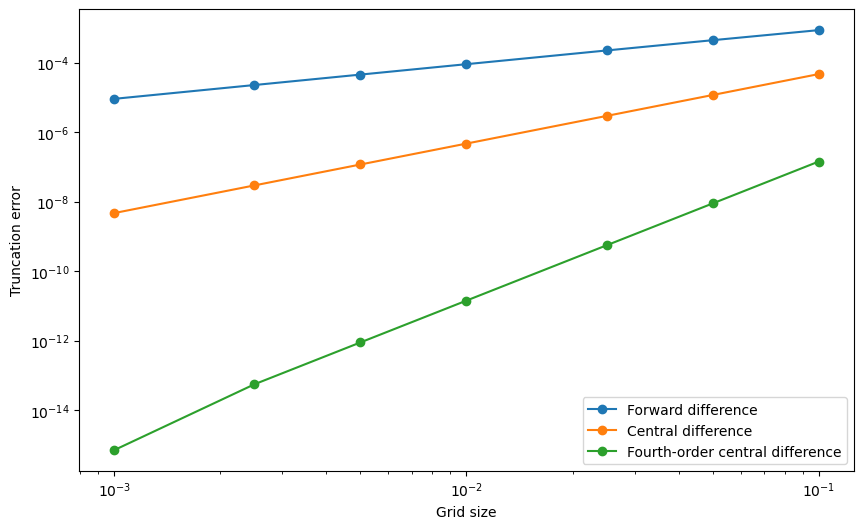
\includegraphics[scale=0.4]{truncation error.png}
    \label{fig:enter-label}
\end{figure}

\newpage
Also the figure of approximation derivate function near the $x=4$ with the grid size $\Delat x = 0.1$ is shown as follows:
\begin{figure}[htpb]
    \centering
    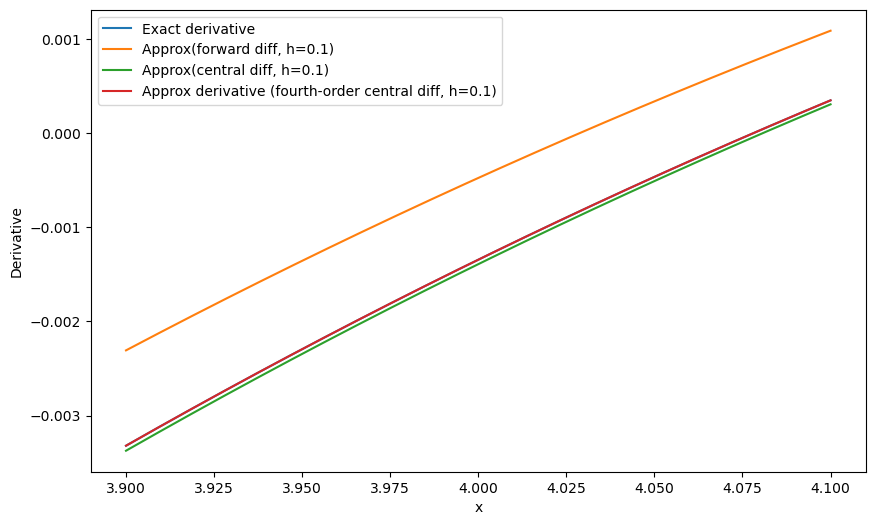
\includegraphics[scale=0.4]{derivate function.png}
    \label{fig:enter-label}
\end{figure}



\end{document}